\chapter{Spanning Trees}
\label{ch:spanning}

\newcommand{\lecnum}{25}
%\newcommand{\lectitle}{Spanning Trees}
\newcommand{\lecturer}{Frank Pfenning, Iliano Cervesato}

\chapterTAGS{application, complexity, graph, traverse-ds, spanning-tree}
\maketitle

\begin{preamble}
\noindent
The following is a simple example of a connected, undirected graph
with 5 vertices ($A, B, C, D, E$) and 6 edges ($AB$, $BC$, $CD$, $AE$,
$BE$, $CE$).
\begin{center}
  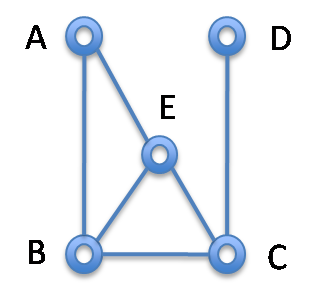
\includegraphics[width=0.3\textwidth]{img/graph1.png}
\end{center}
In this lecture we are particularly interested in the problem of
computing a \emph{spanning tree} for a connected graph.  What is a
tree here?  They are a bit different than the binary search trees we
considered earlier in the course.  One simple definition is that a \emph{tree} is a
\emph{connected graph with no simple cycles}, where a simple cycle is
a path that lets you go from a node to itself without repeating an
edge.  A \emph{spanning tree} for a connected graph $G$ is a tree
containing all the vertices of $G$ and a subset of the edges of $G$.
\end{preamble}

\begin{gram}[Learning Goals]
The corresponding learning goals are as follows:
\begin{description}
\item[Computational Thinking: ]%
  We continue our introduction to graphs by defining spanning trees as
  well as minimum spanning trees for graphs with weighted edges.
\item[Algorithms and Data Structures: ]%
  We examine two ways to compute a spanning tree, and introduce Kruskal's
  algorithm, a classical method for calculating a minimum spanning tree.
\item[Programming: ]%
  We leave the implementation of these algorithms as exercises to the reader.
\end{description}
\end{gram}

\section{Spanning Trees}
\label{sec:spanning:spanning_tree}
\TAGS{graph, traverse-ds, spanning-tree}

Below are two spanning trees for our original example graph ---
there are more.
\begin{center}
  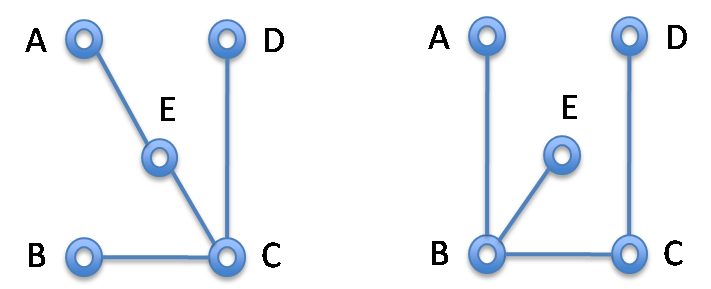
\includegraphics[width=0.6\textwidth]{img/graph2.png}
\end{center}

When dealing with a new kind of data structure, it is a good
strategy to try to think of as many different characterizations
as we can.  This is somewhat similar to the problem of coming
up with good representations of the data; different ones may
be appropriate for different purposes.  Here are some alternative
characterizations:
\begin{enumerate}
\item Connected graph with no cycle (original).
\item Connected graph where no two neighbors are otherwise connected.
  \emph{Neighbors} are vertices connected directly by an edge,
  \emph{otherwise connected} means connected without the connecting
  edge.
\item Two trees connected by a single edge.  This is
  a recursive characterization.  The base case is a single node, with
  the empty tree (no vertices) as a possible special case.
\item A vertex connected to a tree by a single edge.  The base case is
  again a single vertex.  This is another recursive characterization.
\item A connected graph with exactly $v-1$ edges, where $v$ is the
  number of vertices.
\item A graph with exactly one path between any two distinct vertices,
  where a path is a sequence of distinct vertices where each is
  connected to the next by an edge. (For paths in a tree to be
  distinct, we have to disallow paths that double back on themselves).
\end{enumerate}
We call a collection of trees a \emph{forest}.  Naturally, for a graph
with more than one connected component, we will want to compute a
spanning forest consisting of a spanning tree for each connected
component.

% When considering the asymptotic complexity of our various algorithms
% on graphs, it is often useful to categorize graphs as \emph{dense} or
% \emph{sparse}.  Dense graphs have a lot of edges compared to the
% number of vertices.  Writing $v = |V|$ for the number of vertices
% (which will be our notation in the rest of the lecture) we can see
% that the number of edges can be at most $v \times (v-1) / 2$: each
% node could be connected to any other node ($v \times (v-1)$), but in
% an undirected way ($v \times (v-1)/2$).  If we write $e$ for the
% number of edges, we have $e \in O(v^2)$.  By comparison, a tree is
% \emph{sparse} because $e = v-1 \in O(v)$.


\section{Computing a Spanning Tree}
\label{sec:spanning:undirected_algos}
\TAGS{complexity, spanning-tree}

There are many algorithms to compute a spanning tree for a connected
graph.  We will look at two of them.

\subsection{Edge-centric Algorithm}
\label{sec:spanning:undirected_algos:edge_centric}

The first is an example of an \emph{edge-centric} algorithm.  It
leverages definition (3) of trees in the last section.  It proceeds as
follows:
\begin{enumerate}
\item%
  Start with the collection of singleton trees, each with exactly one
  node.
\item%
  As long as we have more than one tree, connect two trees together
  with an edge in the graph.
\end{enumerate}
In the second step, we repeatedly examine one of the original graph
edges and determine whether it spans two disconnected trees.  We can
naively do so by using DFS or BFS to check if its endpoints are
already connected in our spanning forest --- if so we discard the
edge, if not we add it to the spanning tree.  Recall that, with an
adjacency list representation, the complexity of DFS and BFS is
bounded by the number of edges.  The cost of this test is then $O(v)$
because we carry it out \emph{on the trees} which contain at most
$v-1$ edges at any time --- not on the original graph.  How many edges
will we need to examine?  We know by definition (5) of a tree that, if
the graph has $v$ vertices, we will end up adding $v-1$ edges.
However, not all tests are successful!  In the worst case, we will
need to examine all edges in the original graph, i.e., perform the
test $e$ times.  This give this version of the edge-centric algorithm
an $O(ev)$ complexity.

Can we do better?  The efficiency of this algorithm is greatly
affected by how quickly we can tell if an edge would connect two trees
or would connect two nodes already in the same tree.  Using DFS or BFS
to answer this question seems overkill because it does not account for
any information about which node is in which tree --- something we can
track since \emph{we} put them in there.  We will come back to this
question in the next lecture.

\medskip
Let's try this algorithm on our first graph, considering edges in the
listed order:  ($AB$, $BC$, $CD$, $AE$, $BE$, $CE$).
\begin{center}\hspace*{-0.8em}
  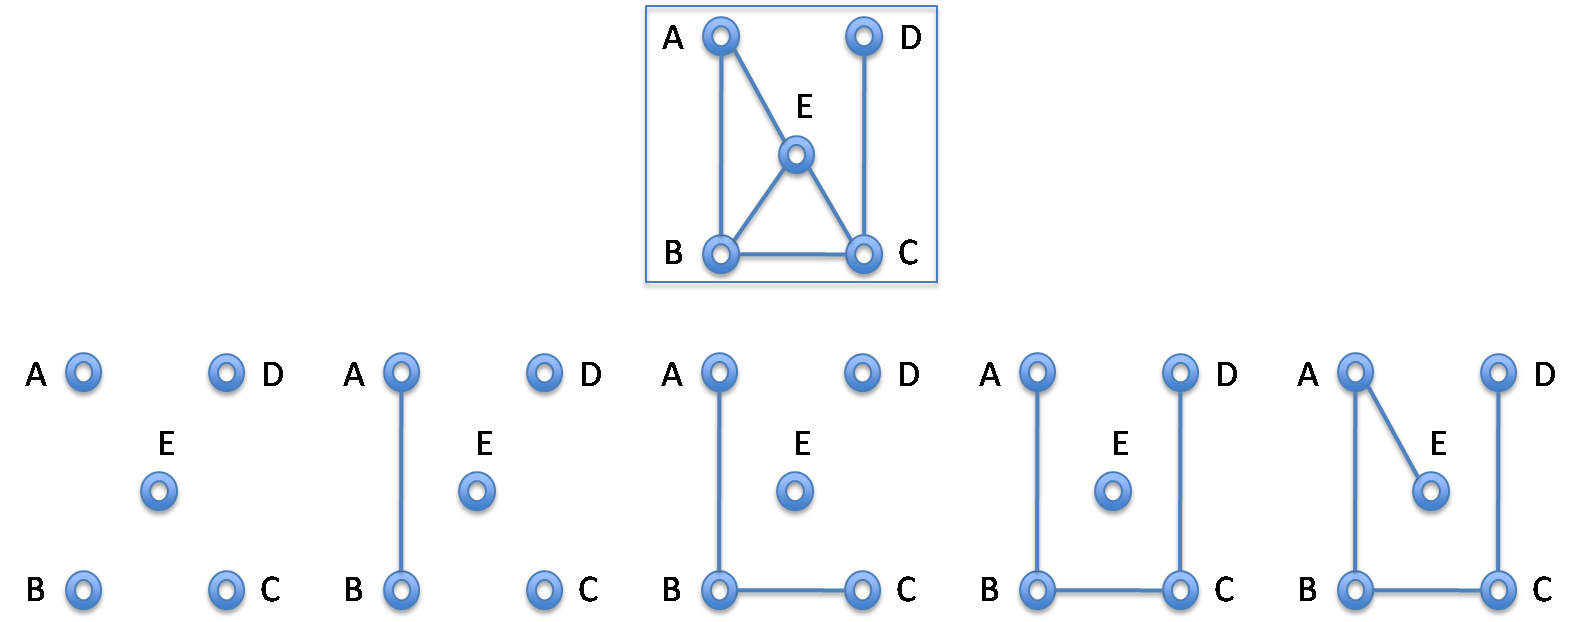
\includegraphics[width=0.99\textwidth]{img/graph3-ec.png}
\end{center}
The given graph is highlighted on top.  The completely disconnected
graph on the left is the starting point for this algorithm.  At the
far right, we have computed a spanning tree, which we know because
we have added $v-1 = 4$ edges.  If we tried to continue, the next edge
$BE$ could not be added because it does not connect two trees, and
neither can $CE$.  The spanning tree is complete.


\subsection{Vertex-centric Algorithm}
\label{sec:spanning:undirected_algos:vertex_centric}

The second algorithm is \emph{vertex-centric}.  It is based on
definition (4) of a tree and proceeds as follow:
\begin{enumerate}
\item Pick an arbitrary node and mark it as being \emph{in the tree}.
\item Repeat until all nodes are marked as \emph{in the tree}:
  \begin{quote}
    Pick an arbitrary node $u$ in the tree with an edge $e$ to a node
    $w$ not in the tree.  Add $e$ to the spanning tree and mark $w$ as
    in the tree.
  \end{quote}
\end{enumerate}
We can implement this by modifying BFS or other algorithm to check
connectivity, where we use a work list (a queue if adapting BFS) to
remember vertices to expand next in step 2.  Specifically, step 1 will
pick an arbitrary vertex and insert it in the queue.  Step 2 will
repeatedly pick a vertex $v$ from the queue and replace it with every
neighbor $w$ that has never been encountered before (which can be
tracked using an array of marks).  At the same time, it will add the
edge $(v,w)$ to the spanning tree.  This will continue as long as
there are vertices in the queue (were the original graph to be
disconnected, we can pick an unmarked node and repeat the algorithm
starting from it, thereby building a spanning forest).

If the original graph is connected, this algorithm has cost $O(e)$ by
an analysis that is identical as that of DFS in the last chapter: for
each vertex it checks whether its neighbors have been visited, which
amounts to two checks for each edge in the graph (one from each
endpoint).  If the original graph is not connected, we will repeat
this procedure for all connected components.  In particular, we will
end up visiting all $v$ vertices --- and nothing else in the
degenerate case of a graph with no edges.  Therefore, this algorithm
has cost $O(\max(v,e))$.   This is better than the
edge-centric algorithm we saw earlier.

Let's play it out on our running example, starting with vertex $A$ and
enqueuing new vertices in alphabetical order:
\begin{center}\hspace*{-0.8em}
  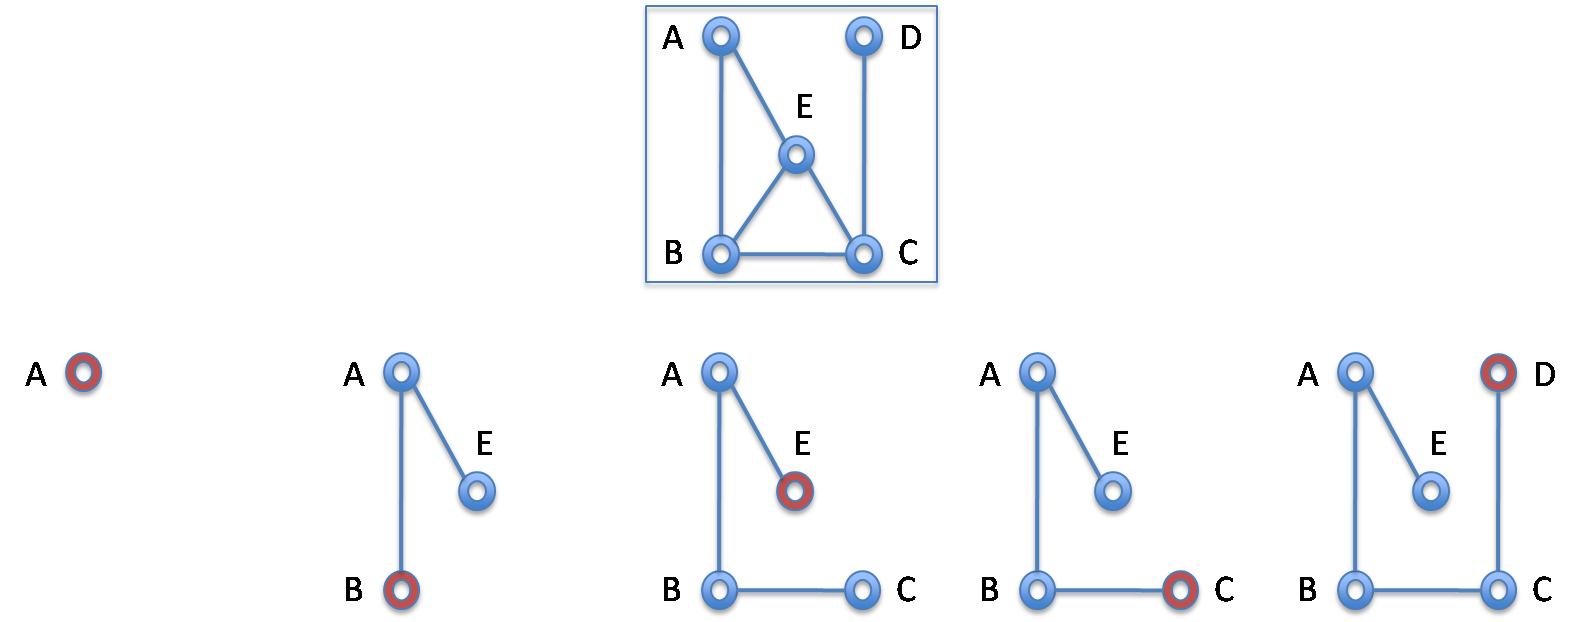
\includegraphics[width=0.99\textwidth]{img/graph3-vc.png}
\end{center}
At each step, the vertex highlighted in red is the node we are
visiting, after dequeuing it but before examining its neighbors.  It
is a coincidence that the resulting spanning tree is identical to the
one we obtained by using the edge-centric algorithm.


\section{Creating a Random Maze}
\label{sec:spanning:maze}
\TAGS{application, spanning-tree}

We can use the algorithm to compute a spanning tree for creating a
random maze.  We start with the graph where the vertices are the cells
and the edges represent the neighbors we can move to in the maze.  In
the graph, all potential neighbors are connected.  A spanning tree
will be defined by a subset of the edges in which all cells in the
maze are still connected by some (unique) path.  Because a spanning
tree connects all cells, we can arbitrarily decide on the starting
point and end point after we have computed it.

How would we ensure that the maze is random?  The idea is to generate
a random permutation (see Exercise~\ref{exc:rand-perm}) of the edges
and then consider the edges in the fixed order.  Each edge is either
added (if it connects two disconnected parts of the maze) or not (if
the two vertices are already connected).  But, of course, we need an
efficient way to determine if the two vertices are already
connected.   The best we can do so far is $O(v)$; we will see in the
next lecture how to do better.


\section{Minimum Weight Spanning Trees}
\label{sec:spanning:mst}
\TAGS{complexity, graph, spanning-tree}

In many applications of graphs, there is some measure associated with
the edges.  For example, when the vertices are locations then the edge
weights could be distances.  We might then be interested in not any
spanning tree, but one whose total edge weight is minimal among all
the possible spanning trees, a so-called \emph{minimum weight spanning
  tree} (MST).  An MST is not necessarily unique.  For example, all
the edge weights could be identical in which case any spanning tree
will be minimal.

We annotate the edges in our running example with edge weights
as shown on the left below.  On the right is the minimum weight
spanning tree, which has weight 9.
\begin{center}
  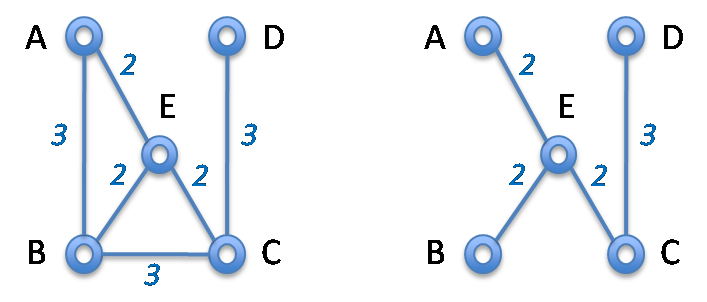
\includegraphics[width=0.6\textwidth]{img/graph4.png}
\end{center}

Before we develop a refinement of our edge-centric algorithm for
spanning trees to take edge weights into account, we discuss a basic
property it is based on.

\bigskip
\noindent
\textbf{Cycle Property.}
\begin{quote}
  Let $C$ be a simple cycle in graph $G$, and $e$ be an edge of
  maximal weight in $C$.  Then there is some MST of $G$ that does not
  contain $e$.
\end{quote}

How do we convince ourselves of this property?  Assume we have a
minimum spanning tree $T$, and edge $e$ from the cycle property
connects vertices $u$ and $w$.  If $e$ is not in $T$, then, indeed, we
don't need it.  If $e$ is in $T$, we will construct another spanning
tree without $e$ of weight less than or equal to $T$'s
weight. Removing edge $e$ splits $T$ into two subtrees.  There must be
another edge $e'$ from $C$ that is not in $T$ which also connects the
two subtrees.  Removing $e$ and adding $e'$ instead yields another
spanning tree, $T'$, which does not contain $e$.  $T'$ has equal or
lower weight to $T$, since $e'$ must have weight less than or equal to
$e$.

The cycle property is the basis for \emph{Kruskal's algorithm}.
\begin{enumerate}
\item%
  Sort all edges in increasing weight order.
\item%
  Consider the edges in order.  If the edge does not create a cycle,
  add it to the spanning tree.  Otherwise discard it.  Stop when $v-1$
  edges have been added, because then we must have a spanning tree.
\end{enumerate}
Why does this create a minimum-weight spanning tree?  It is a
straightforward application of the cycle property (see
Exercise~\ref{exc:kruskal}).

Sorting the edges will take $O(e\log e)$ steps with most appropriate
sorting algorithms.  The complexity of the second part of the
algorithm depends on how efficiently we can check if adding an edge
will create a cycle or not.  So far, the best we can do is $O(ev)$.
%   As we will see in the next lecture, this
% can be $O(e\log v)$ or even more efficient if we use a so-called
% \emph{union-find} data structure.

Illustrating the algorithm on our example
\begin{center}
  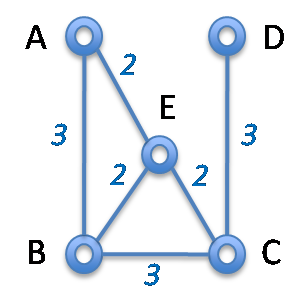
\includegraphics[width=0.3\textwidth]{img/graph5.png}
\end{center}
we first sort the edges.  There is some ambiguity --- say we
obtain the following list
\[\begin{array}{cc}
AE & 2 \\
BE & 2 \\
CE & 2 \\
BC & 3 \\
CD & 3 \\
AB & 3
\end{array}\]
We now add the edges in order, making sure we do not create
a cycle.  After $AE$, $BE$, $CE$, we have
\begin{center}
  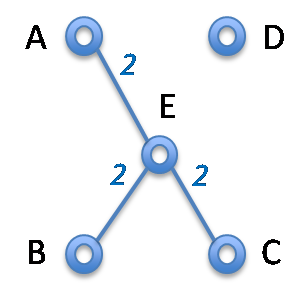
\includegraphics[width=0.3\textwidth]{img/graph6.png}
\end{center}
At this point we consider $BC$.  However, this edge would
create a cycle $BCE$ since it connects two vertices in the
same tree instead of two different trees.  We therefore
do not add it to the spanning tree.  Next we consider $CD$,
which does connect two trees.  At this point we have a
minimum spanning tree
\begin{center}
  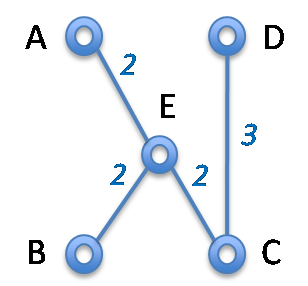
\includegraphics[width=0.3\textwidth]{img/graph7.png}
\end{center}
We do \emph{not} consider the last edge, $AB$, because we have already
added $v-1 = 4$ edges.

In the next lecture we will analyze the problem of incrementally
adding edges to a tree in a way that allows us to quickly determine if
an edge would create a cycle.

Kruskal's algorithm is nothing more than the edge-centric algorithm
examined in Section~\ref{sec:spanning:undirected_algos}, preceded by
the additional step of sorting the edges by increasing weight (and
examining edges on the basis of that order).  The vertex-centric
algorithm can similarly be adapted to compute a minimum spanning tree
of a weighted graph.  At each step, of all edges between vertices in
the tree and vertices outside the tree, we will add an edge of minimal
weight.  To this end, when visiting a vertex $v$, we cannot put down
the edge $(v,w)$ to an unvisited neighbor $w$ since there may be a
cheaper way to get to $w$.  Instead, we will record these edges
(rather than just the vertices) not in a queue but in a \emph{priority
  queue} with lighter edges having priority over heavier edges.  A step now
consists in retrieving an edge of minimal weight from the priority
queue: if its endpoint is already in the spanning tree we discard it
(we have already found a cheaper way to get to that vertex), otherwise
we add it (and insert its unvisited neighbors in the priority queue).
The resulting procedure is known as \emph{Prim's algorithm} and its
run time complexity is dominated by the cost of inserting edges in the
priority queue.  This cost is $O(e \log e)$ since we may be inserting
all edges in the priority queue.


%\clearpage
\section{Exercises}
\label{sec:spanning:exercises}

\begin{exercise}[Randomizing an Array]
\label{exc:rand-perm}
Write a function to generate a random permutation of a given array,
using a random number generator with the interface in the standard
\lstinline'rand' library.  What is the asymptotic complexity of your
function?
\end{exercise}

\begin{exercise}[Proving Correctness]
\label{exc:kruskal}
Prove that the cycle property implies the correctness of Kruskal's
algorithm.
\end{exercise}

% \clearpage
% \bibliographystyle{alpha}
% \bibliography{modal}

% \cleardoublepage
